\chapter{Реализация и сравнительное тестирование системы.}

В данном разделе представлено комплексное описание реализации и тестирования системы. Рассмотрен процесс программирования основных компонентов и их интеграции в общую архитектуру. Рассмотрены детали реализаций микросервисов, на которые будут приходить запросы. Объяснено как развертываются компоненты в кластере. Особое внимание уделено способу сбора трассировки, настройке сборщика данных и конфигурации Jaeger. Разъясняется конфигурация service mesh в Istio, в сравнении с самостоятельно реализованной альтернативой. Описаны методики тестирования, позволяющие оценить производительность и отказоустойчивость системы. Приводятся результаты эксперементов нагрузочного тестирования. Строятся, сравниваются и объясняются графики задержек в каждой из реализаций.  Рассмотрены перспективы и возможности дальнейшнего развития исследования.



\section{Состав и структура реализованного программного обеспечения}


% В данной главе описана структура реализованного программного обеспечения, в основе которого лежит микросервисная архитектура, развернутая на кластере виртуальных машин с использованием k3s. Написан шаблон Python кода сервера (\ref{lst:server.py}), реализована версии с Istio, написана библиотека с реализацией паттерна Circuit Breaker. Для реализации веб-сервисов использован Flask, запущенный через Gunicorn для повышения производительности, что позволяет эффективно обрабатывать входящие запросы. Все компоненты упакованы в Docker-образы и опубликованы на Docker Hub. Приведён листинг Docker-файла сервера (\ref{lst:dockerfile-server}), а так же листинг Docker-файла прокси-сервера (\ref{lst:dockerfile-proxy}).

% Развертывание компонентов системы осуществляется посредством Helm-чартов, где все параметры заданы в файле values.yaml (\ref{lst:values}). Такой подход обеспечивает гибкую конфигурацию и автоматизацию обновлений, позволяя централизованно управлять параметрами развертывания в кластере. 

Реализовано программное обеспечение, базирующееся на микросервисной архитектуре, развернутой в отдельном кластере виртуальных машин с использованием облегчённой платформы Kubernetes - k3s. Для каждой из рассматриваемых версий системы (с применением Istio и без него) был создан собственный кластер k3s. Каждый класер развернут на отдельных физических серверах.
Каждая виртуальная машина в составе кластера конфигурировалась с выделением 2 процессорных ядер и 4 ГБ оперативной памяти. При этом кластер построен по схеме «один сервер — два агента»: серверная роль выполнялась первой виртуальной машиной, а две другие были агентами.
Архитектура системы с Istio включает следующие компоненты:
\begin{itemize} 
  \item Главный сервер, реализованный на языке Python с использованием фреймворка Flask и запускаемый через Gunicorn для эффективного параллельного обслуживания запросов;
  \item Прокси сервер, также основанный на Python и Flask, на который запросы изначально поступают;
  \item Сервис трассировки Jaeger v2, включающий компоненты пользовательского интерфейса (Jaeger UI) и HTTP-сервиса для сбора и отображения трассировок;
  \item Компоненты Fluent Bit, развернутые в режиме DaemonSet на каждом узле для сбора и аггрегации логов;
  \item Istio Sidecar, управляющий межсервисными коммуникациями и реализующий функции шаблона Circuit Breaker;
  \item средство нагрузочного тестирования K6, запускаемое в виде задания (Job) в кластере Kubernetes.
\end{itemize}

Версия системы без Istio сохраняет аналогичную структуру и состав компонентов, исключая наличие sidecar контейнера Istio Sidecar и соответствующих механизмов ingress и egress, обеспечиваемых этим сервисом.
Все компоненты системы упакованы в Docker контейнеры и размещены в открытом доступе на \href{https://hub.docker.com/repositories/robocatt}{Docker Hub}. Листинги Docker файлов для основного и прокси сервера приведены в приложении (см. \ref{lst:docker-server-istio} и \ref{lst:docker-client-istio}).
Для автоматизации процесса развертывания, конфигурирования и обновления компонентов используются Helm-чарты, параметры которых централизованно управляются посредством файла values.yaml (см. \ref{lst:values-istio}). Такой подход позволяет гибко и эффективно управлять параметрами среды исполнения и автоматизировать операции развертывания системы


\section{Основные сценарии использования реализованных решений}
Библиотека Circuit Breaker была создана с целью повышения отказоустойчивости распределённых приложений, особенно в случаях, когда применение полнофункционального решения, такого как Istio, избыточно. Предлагаемая библиотека может легко интегрироваться в различные микросервисные архитектуры, позволяя эффективно управлять состоянием запросов и обрабатывать ошибки взаимодействия между компонентами системы.
Особенностью библиотеки является её простота и минимальное влияние на производительность приложений, что подтверждается проведёнными испытаниями (см. главу 4.3). Применение данной библиотеки позволяет существенно ускорить работу микросервисных архитектур за счёт устранения излишней нагрузки на промежуточные прокси-сервисы.
Помимо реализации Circuit Breaker была разработана удобная система трассировки, представленная JSON-экспортером, который пишет данные trace в стандартный поток вывода (stdout). Данный подход позволяет избежать лишних затрат процессорных ресурсов на передачу трассировочных данных напрямую и интегрироваться с такими инструментами, как Fluent Bit, для последующей обработки и анализа. Экспортер полностью совместим с протоколами OpenTelemetry и может быть легко добавлен в уже существующую инфраструктуру, использующую Jaeger, с минимальными изменениями в коде приложения:
\begin{verbatim}
from otlp_json_console_exporter import OTLPJsonConsoleExporter
json_exporter = OTLPJsonConsoleExporter()
provider.add_span_processor(BatchSpanProcessor(json_exporter))
\end{verbatim}
Таким образом, предложенные решения не только обеспечивают простоту интеграции и использования паттерна Circuit Breaker, но и предоставляют эффективные инструменты для оценки и анализа задержек в существующих архитектурах. Полный листинг кода JSON-экспортера приведён в приложении (см. \ref{lst:otlp_json_conole_exporter}).


\section{Результаты тестирования}

В рамках тестирования были проведены испытания системы согласно сценариям, описанным в разделе~\ref{sec:test-analysis}. В частности, выполнены следующие тесты:
\begin{itemize}
\item \textbf{Тест работоспособности библиотеки Circuit Breaker.} Проведено испытание с помощью инструмента k6 и визуализации в Lens, подтвердившее корректное срабатывание блокировки обращений после трёх неудачных попыток запросов к несуществующему адресу (HTTP 404) (см. \ref{pic:CB-work}). После достижения заданного порога система блокирует доступ к целевому серверу на 30 секунд, обеспечивая устойчивость к повторяющимся сбоям.




\begin{figure}[htbp]
  \centering
  
  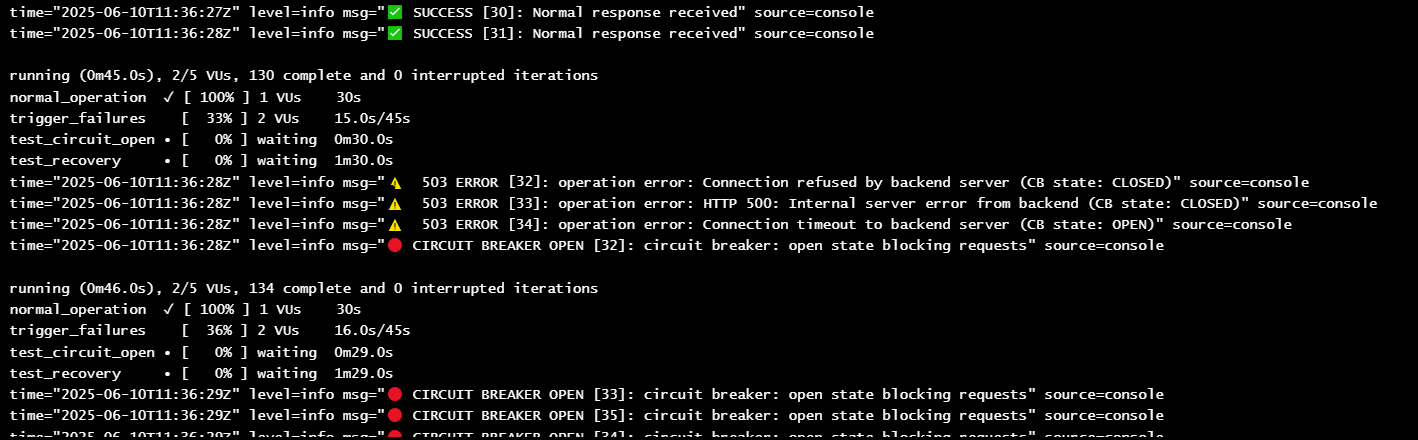
\includegraphics[
      width=\linewidth,            % never wider than text block
      height=0.8\textheight,       % never taller than 80 % of the text body
      keepaspectratio              % obey aspect ratio
  ]{img/CB_work_example.png}
  \caption{Лог k6 об успешном применении Circuit Breaker}
  \label{pic:CB-work}
\end{figure}

\item \textbf{Нагрузочное тестирование с различным числом виртуальных пользователей (vus).} Проведены испытания с постепенным увеличением нагрузки, при котором количество пользователей варьировалось в пределах 5, 10, 25 и 50 vus. Каждый тест длился три минуты, состоял из трех этапов: постепенного нарастания нагрузки в течение первых 30 секунд, поддержание пикового уровня нагрузки в течение последующих двух минут и завершающий 30-секундный период постепенного снижения нагрузки.
\item \textbf{Тестирование с увеличением размера передаваемого запроса.} Также проведено тестирование производительности при постепенном увеличении размера передаваемых запросов до 1, 5, 100 и 500 КБ при фиксированном количестве виртуальных пользователей (10 vus). Каждый тест также состоял из трёх этапов: начального нарастания нагрузки в течение 30 секунд, поддержания нагрузки на максимальном уровне в течение двух минут и завершающего 30-секундного этапа плавного снижения нагрузки.
\end{itemize}

Для анализа задержек и оценки времени отклика использовалась система трассировки Jaeger, один trace которой состоит из 11 spans, представленных на диаграмме \ref{pic:trace-struct}. 

\begin{figure}[htbp]
  \centering
  
  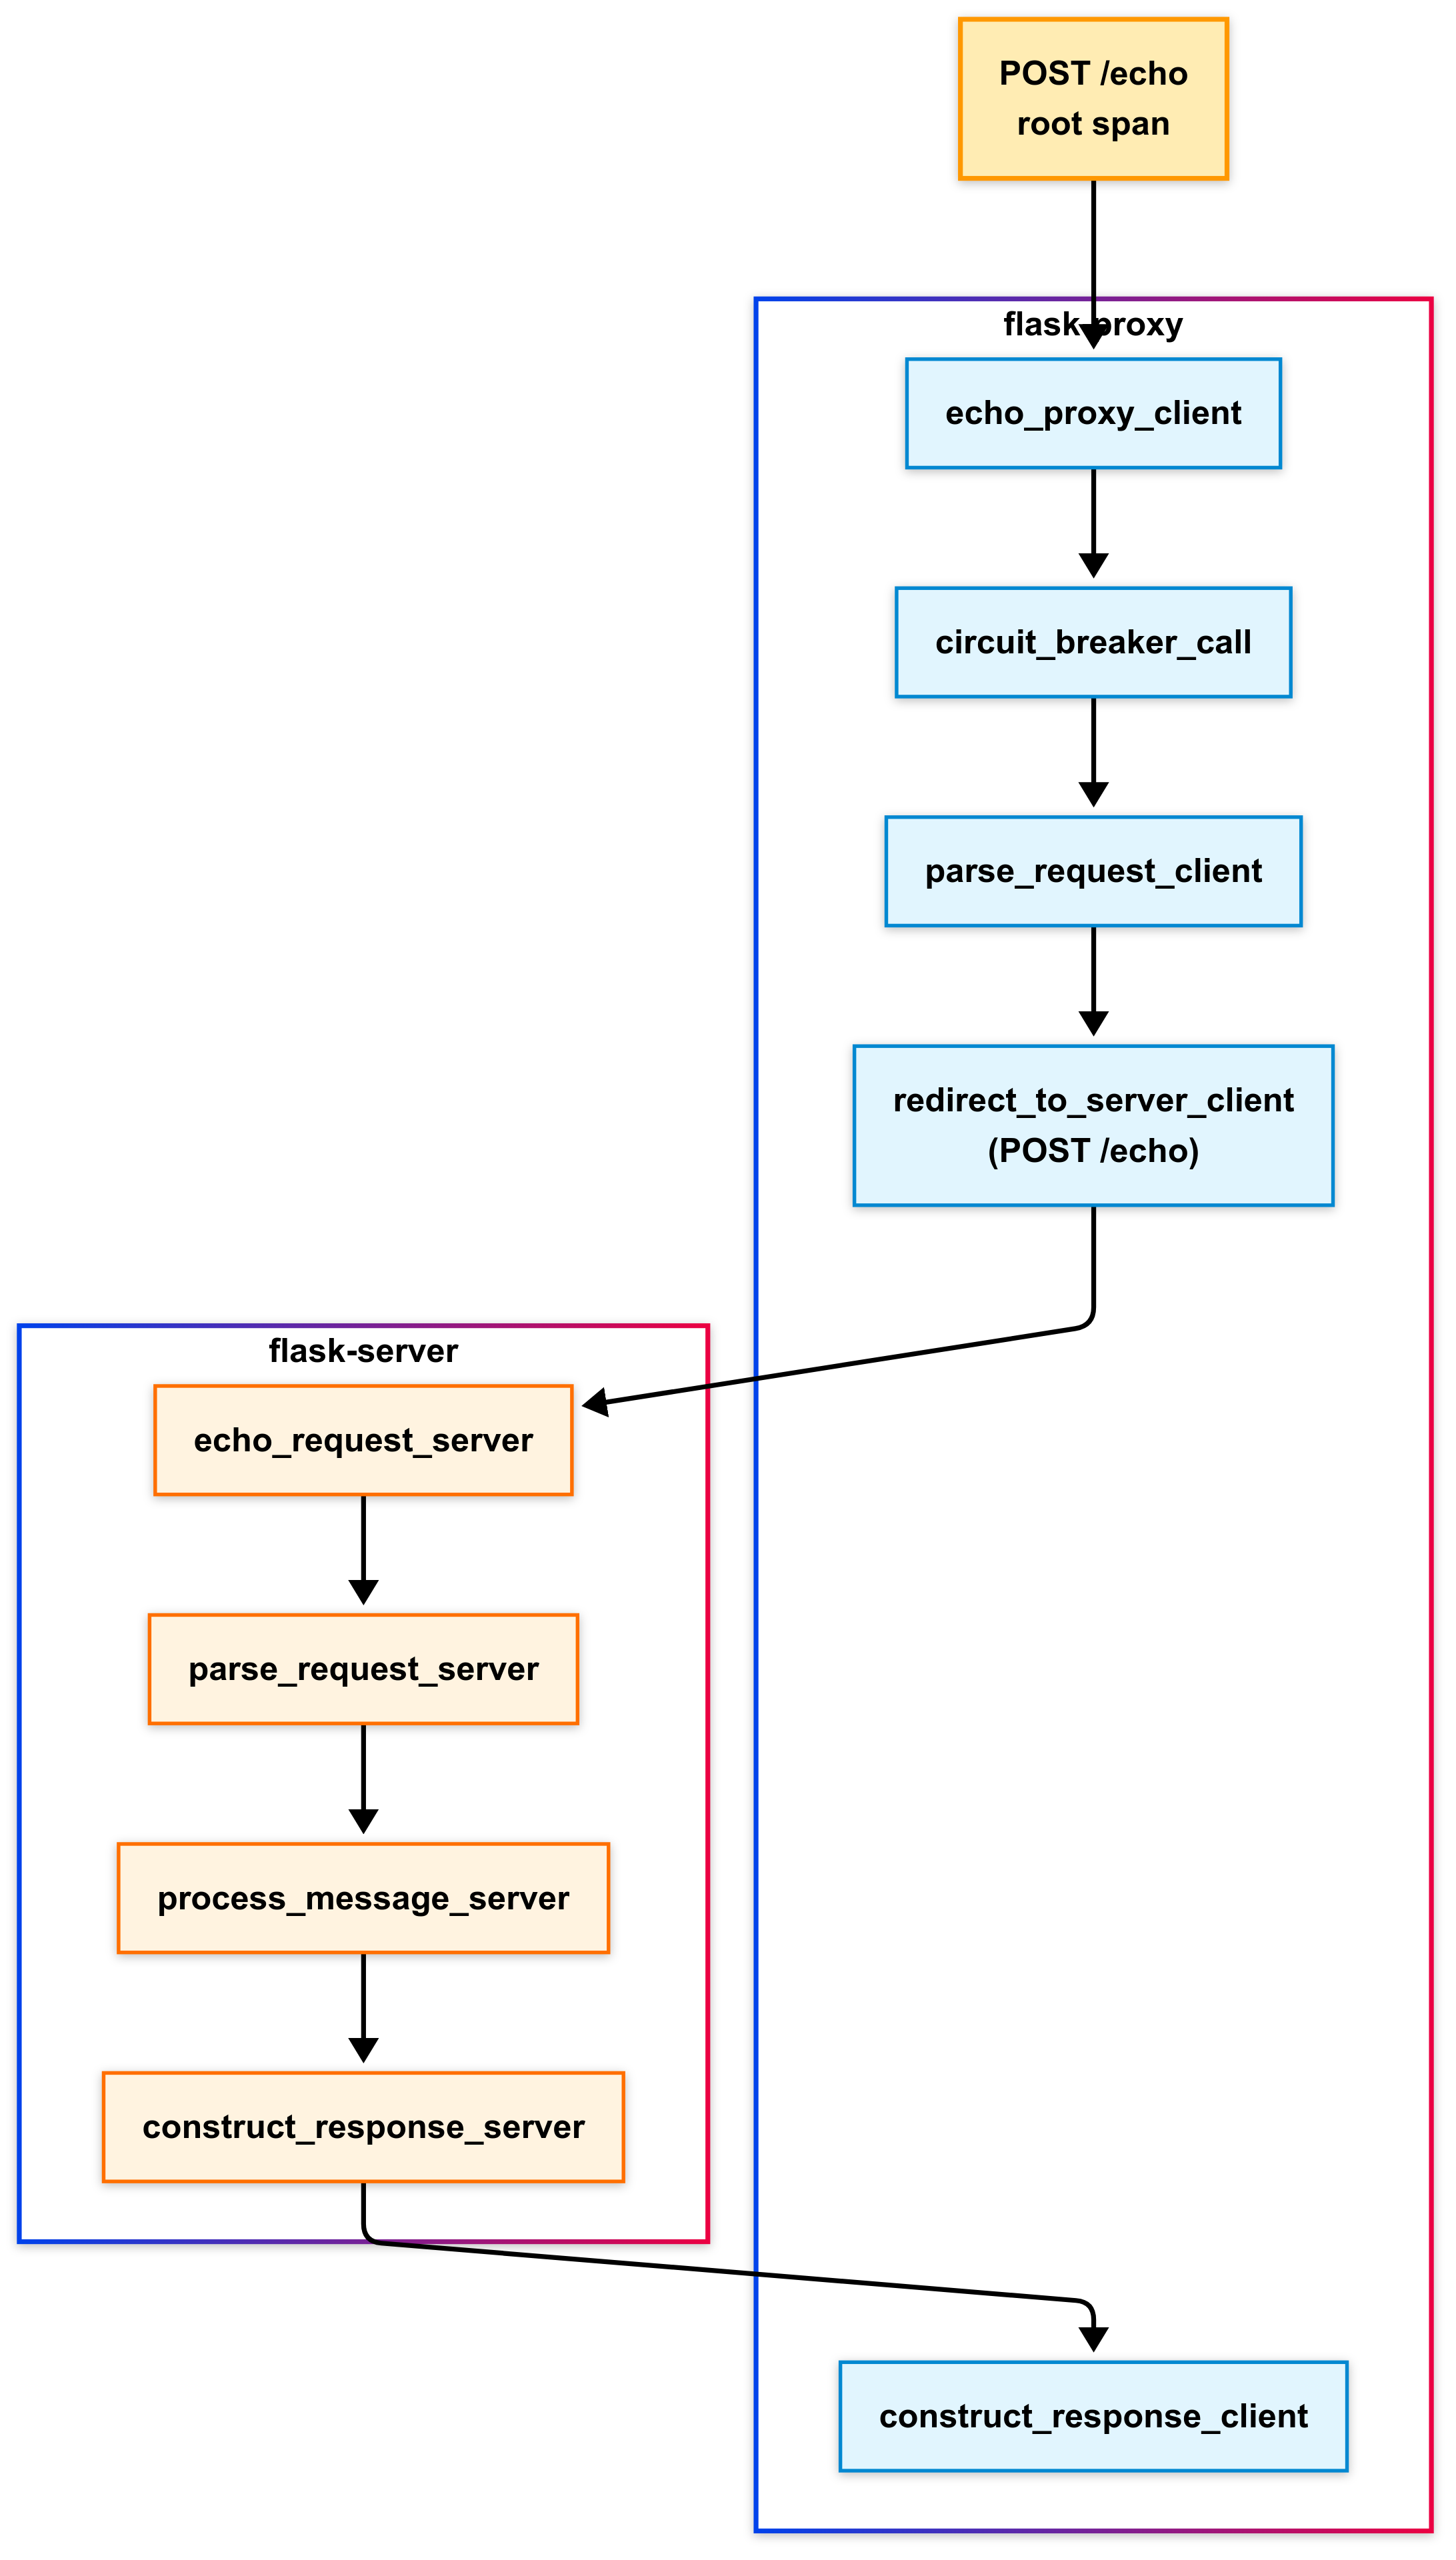
\includegraphics[
      width=\linewidth,            % never wider than text block
      height=0.8\textheight,       % never taller than 80 % of the text body
      keepaspectratio              % obey aspect ratio
  ]{img/trace_struct.png}
  \caption{Описание структуры trace.}
  \label{pic:trace-struct}
\end{figure}

Trace состоит из следующих спанов:
\begin{itemize}
\item \textbf{root span (POST /echo)} – корневой span, обозначающий начальную точку обработки запроса.
\item \textbf{echo\_proxy\_client} – обработка запроса на прокси-сервере.
\item \textbf{circuit\_breaker\_call} – span, отражающий логику работы Circuit Breaker.
\item \textbf{parse\_request\_client} – span, обозначающий разбор запроса на прокси.
\item \textbf{redirect\_to\_server\_client (POST /echo)} – перенаправление запроса на сервер.
\item \textbf{construct\_response\_client} – формирование ответа клиенту на прокси.
\item \textbf{echo\_request\_server} – принятие запроса сервером.
\item \textbf{parse\_request\_server} – разбор запроса на сервере.
\item \textbf{process\_message\_server} – непосредственная обработка сообщения на сервере.
\item \textbf{construct\_response\_server} – формирование ответа сервером.
\end{itemize}

На диаграмме (см. \ref{pic:trace-flow}) представлено формирование спанов в Python-коде и последующая их агрегация в базе данных Jaeger v2.

\begin{figure}[htbp]
  \centering
  
  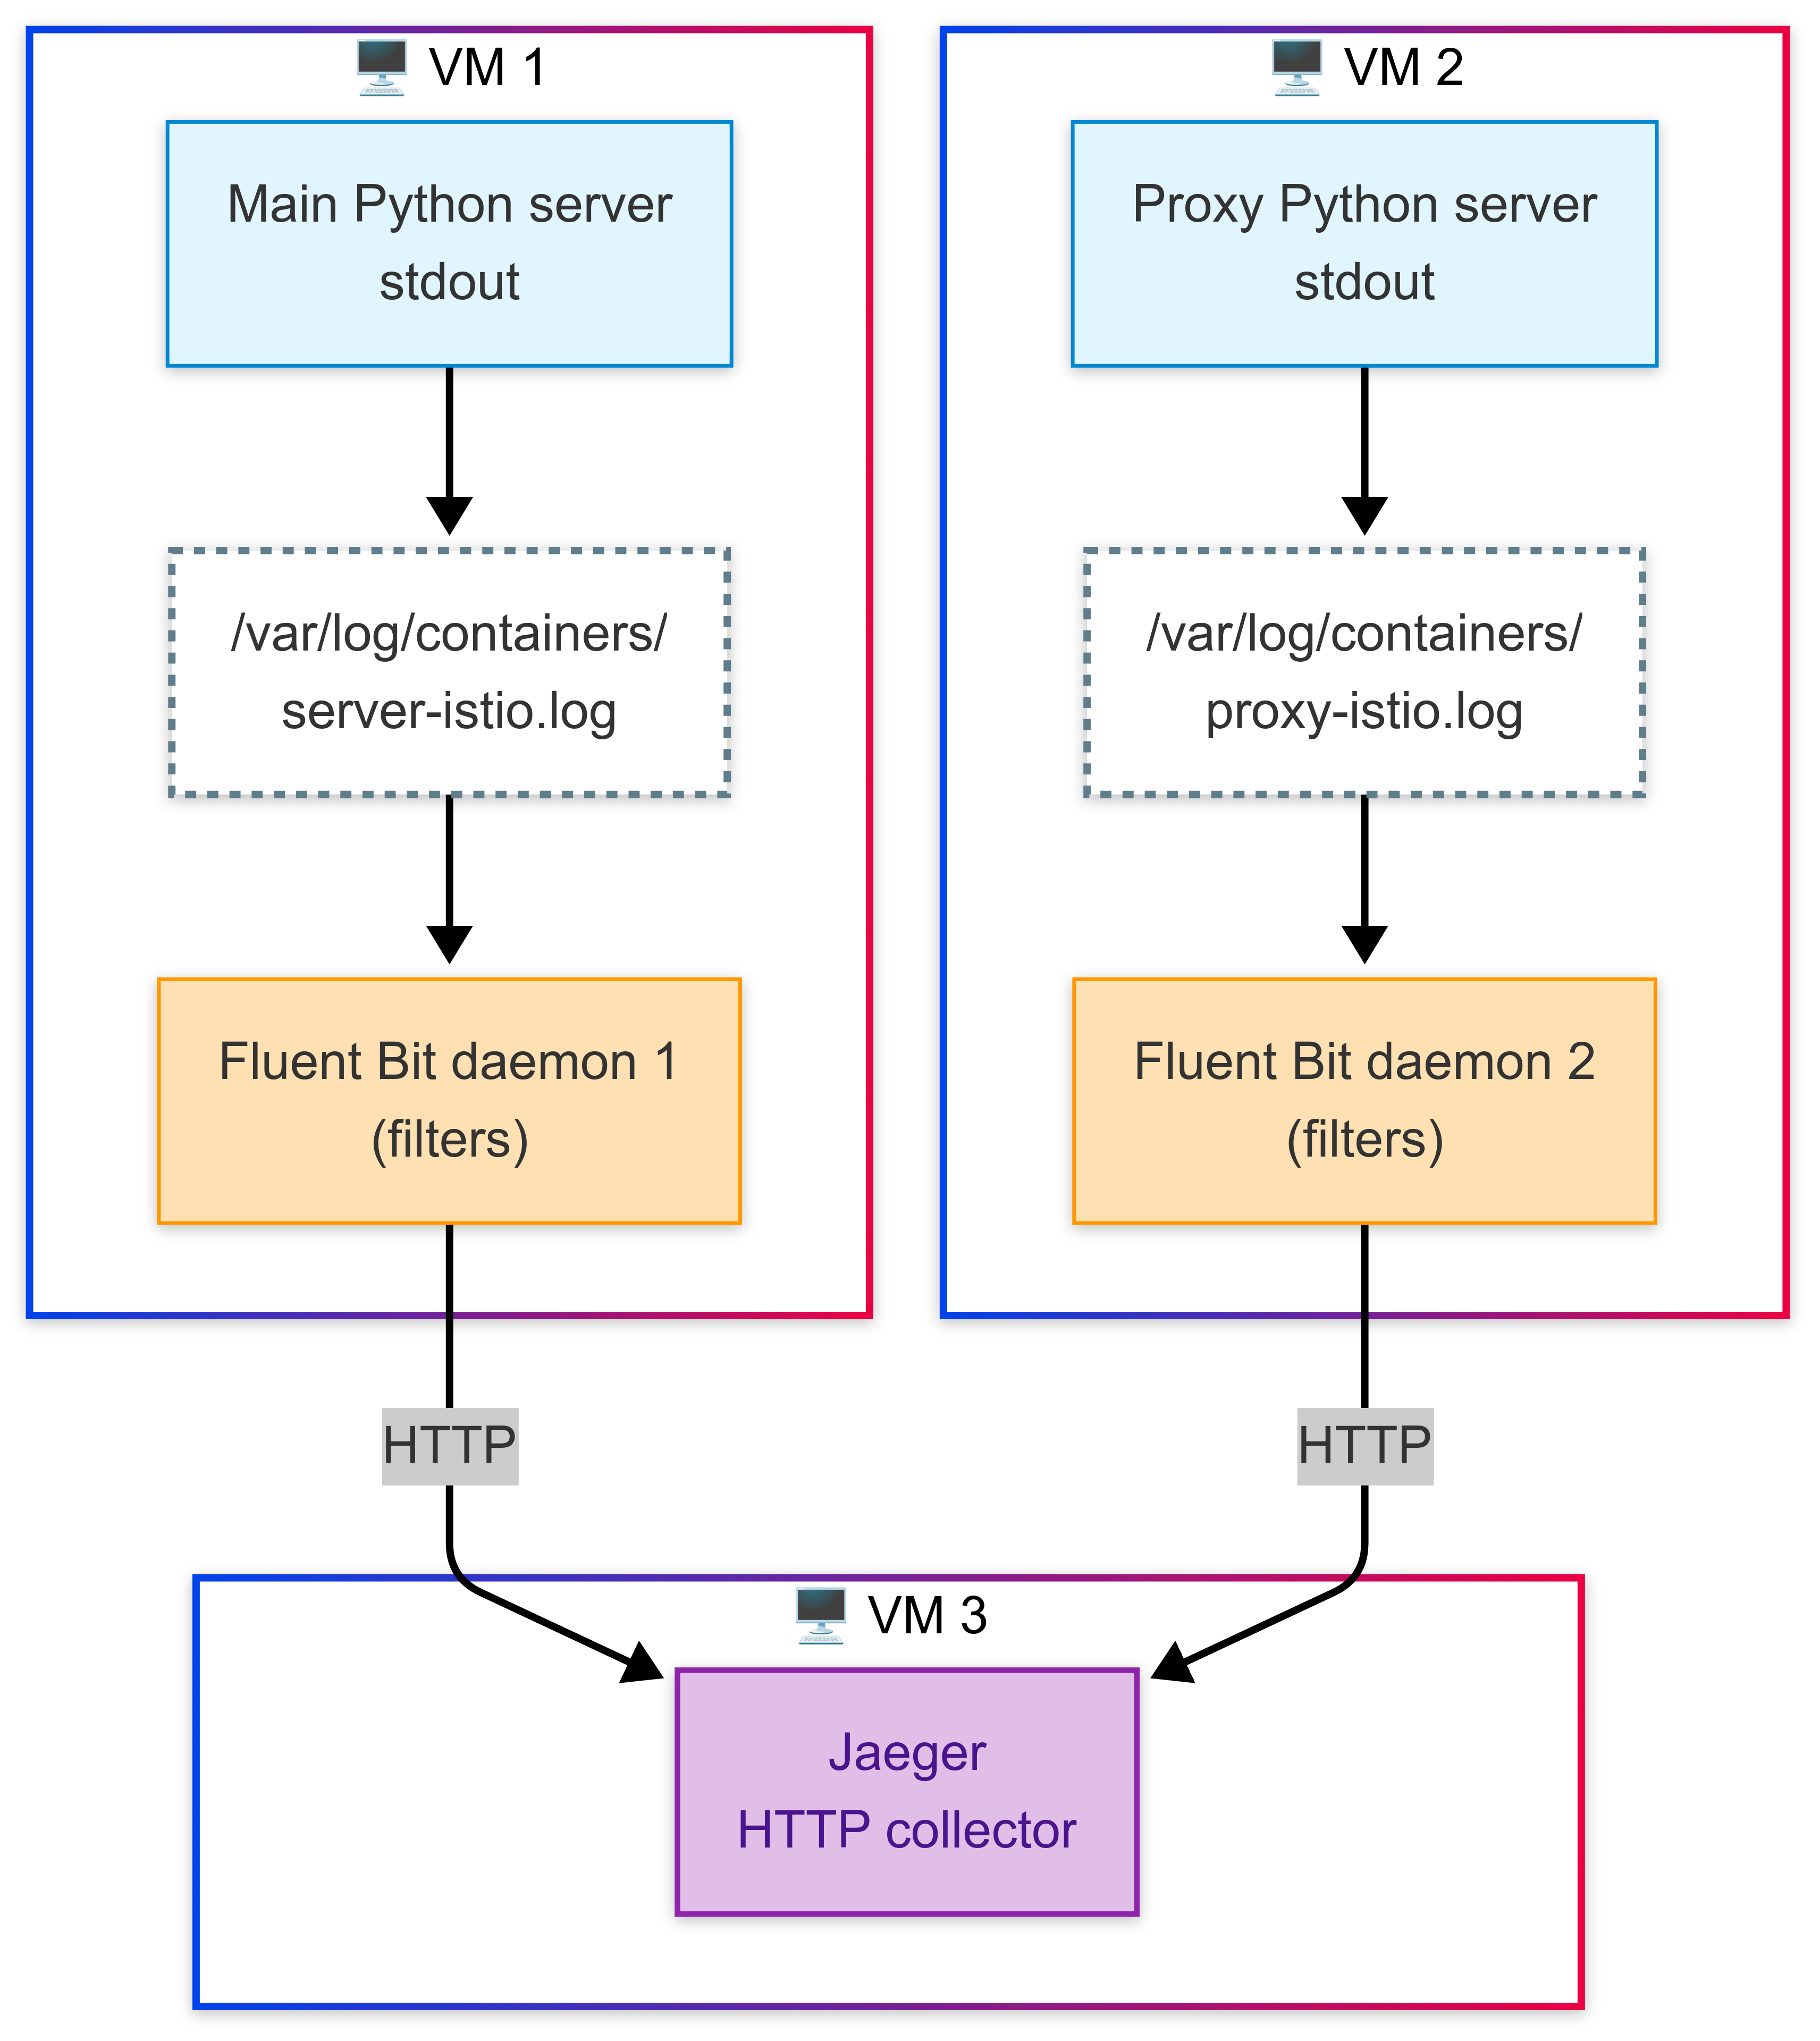
\includegraphics[
      width=\linewidth,    
      height=0.8\textheight,
      keepaspectratio              % obey aspect ratio
  ]{img/trace_flow.png}
  \caption{Описание формирования trace.}
  \label{pic:trace-flow}
\end{figure}

\FloatBarrier 

По результатам нагрузочного тестирования построена диаграмма распределения задержек в зависимости от количества виртуальных пользователей (см. рис. \ref{pic:trace_duration_subplots}). Данная диаграмма отражает сравнительную производительность реализации с использованием Istio и без него. На примере обработки 50 виртуальных пользователей видно, что сервер испытывает значительную нагрузку, и паттерн Circuit Breaker в этих условиях позволяет быстрее отвечать на запросы, в то время как собственная реализация демонстрирует значительно меньшие задержки.
Более наглядное сравнение показывает столбчатая диаграмма (см. рис. \ref{pic:mean_trace_duration_vs_vus}), где реализация с Istio характеризуется примерно на 20\% большей задержкой независимо от количества виртуальных пользователей.




\begin{figure}[htbp]
  \centering
  
  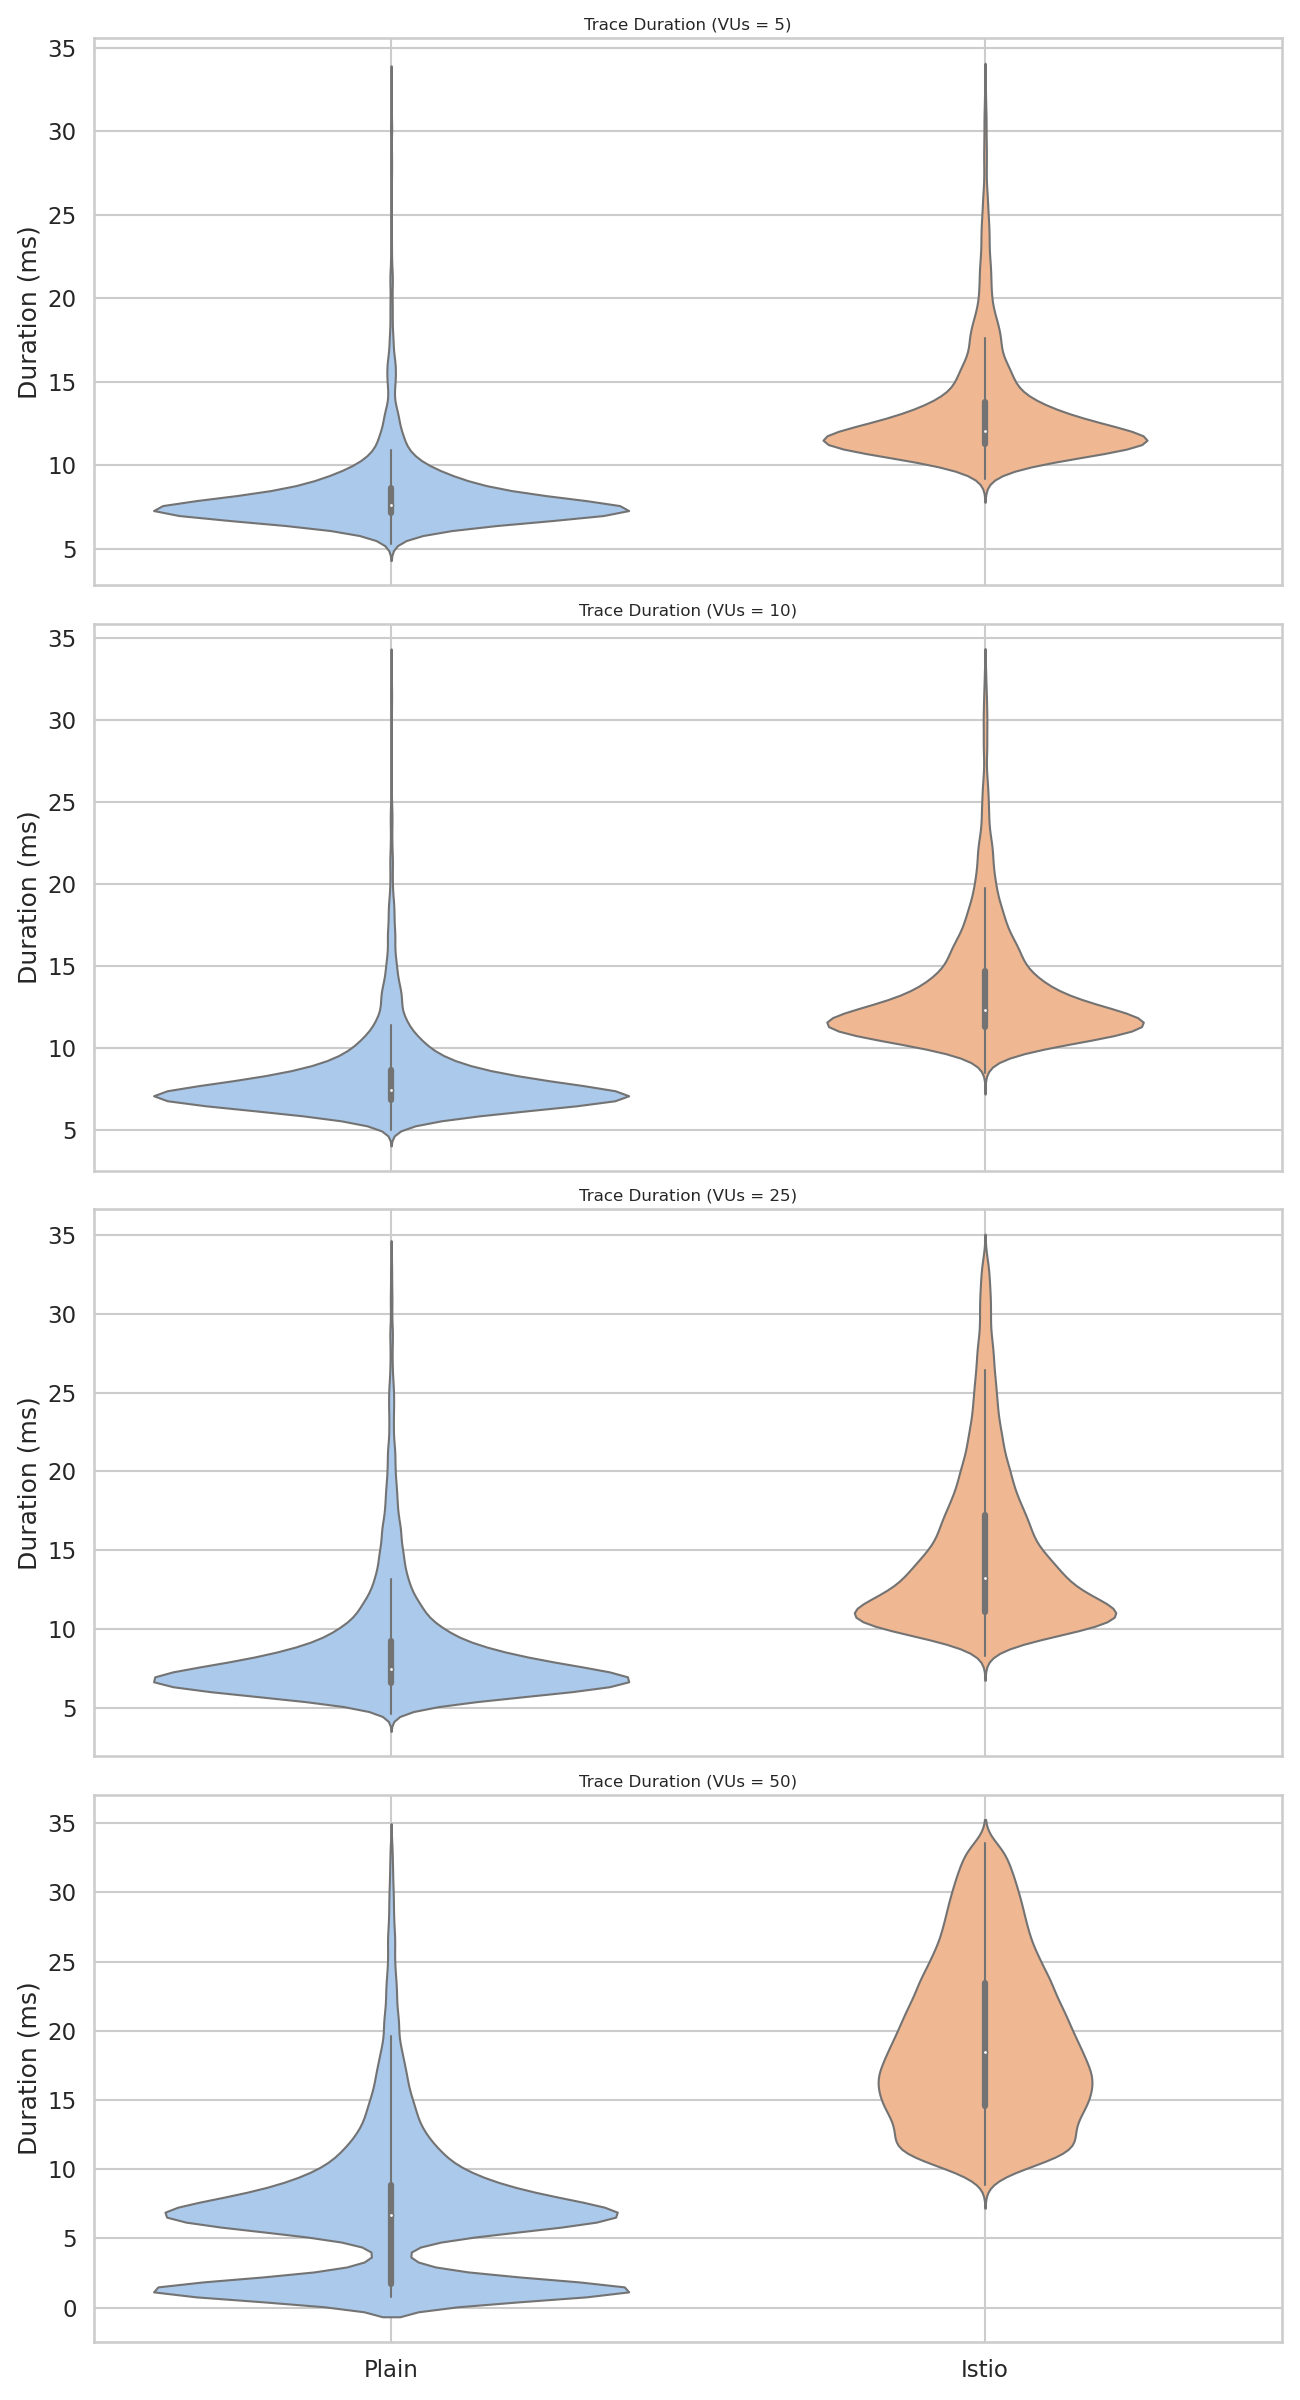
\includegraphics[
      width=\linewidth,            % never wider than text block
      height=0.8\textheight,       % never taller than 80 % of the text body
      keepaspectratio              % obey aspect ratio
  ]{img/trace_duration_subplots.png}
  \caption{Диаграмма распределения задержек в зависимости от количества виртуальных пользователей. }
  \label{pic:trace_duration_subplots}
\end{figure}


\begin{figure}[htbp]
  \centering
  
  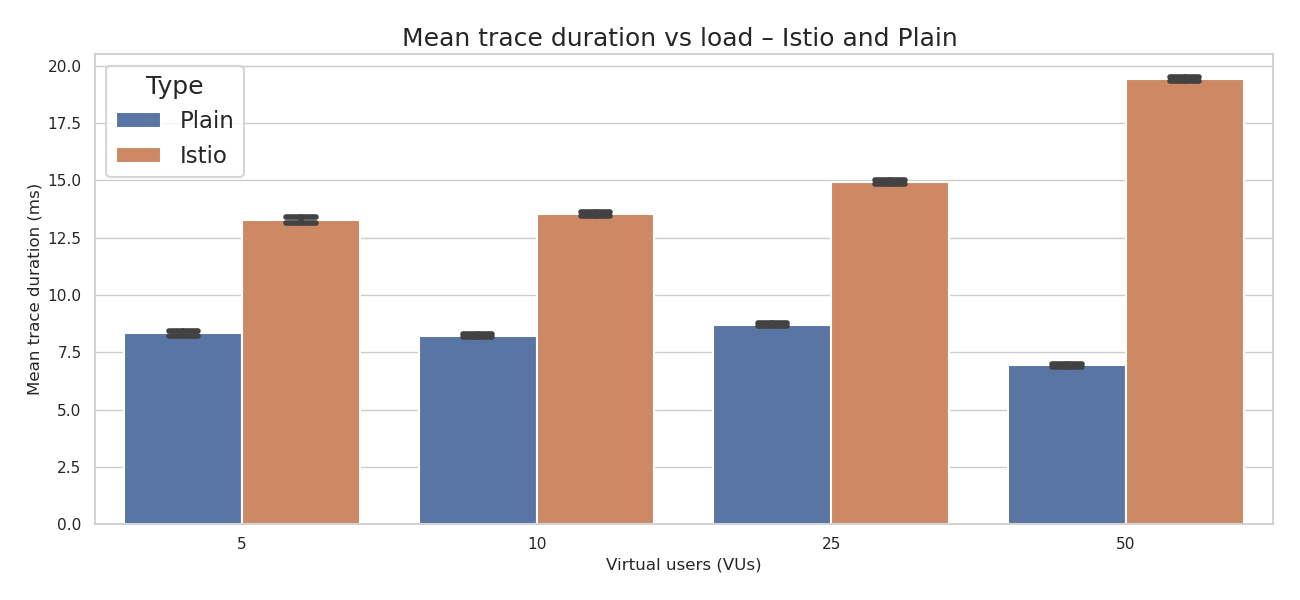
\includegraphics[
      width=\linewidth,            % never wider than text block
      height=0.8\textheight,       % never taller than 80 % of the text body
      keepaspectratio              % obey aspect ratio
  ]{img/mean_trace_duration_vs_vus.png}
  \caption{Среднее время выполнения trace в зависимости от числа виртуальных пользователей. }
  \label{pic:mean_trace_duration_vs_vus}
\end{figure}

\FloatBarrier 

Дополнительно проведены тесты с различным размером полезной нагрузки (payload). Эти тесты подтвердили работоспособность предложенного решения при любых объёмах данных, а также показали незначительность влияния размера полезной нагрузки на относительную производительность обеих реализаций (см. рис. \ref{pic:mean_trace_duration_vs_payload}).
На рисунке \ref{pic:span_latency_100kb} представлена столбчатая диаграмма среднего времени выполнения отдельных спанов в тесте с payload размером 100 КБ. Заметно, что спаны, требующие сетевого взаимодействия, демонстрируют разницу в скорости между двумя реализациями, в то время как операции, выполняемые исключительно процессором, имеют одинаковую производительность в обоих случаях.

 \begin{figure}[htbp]
  \centering
  
  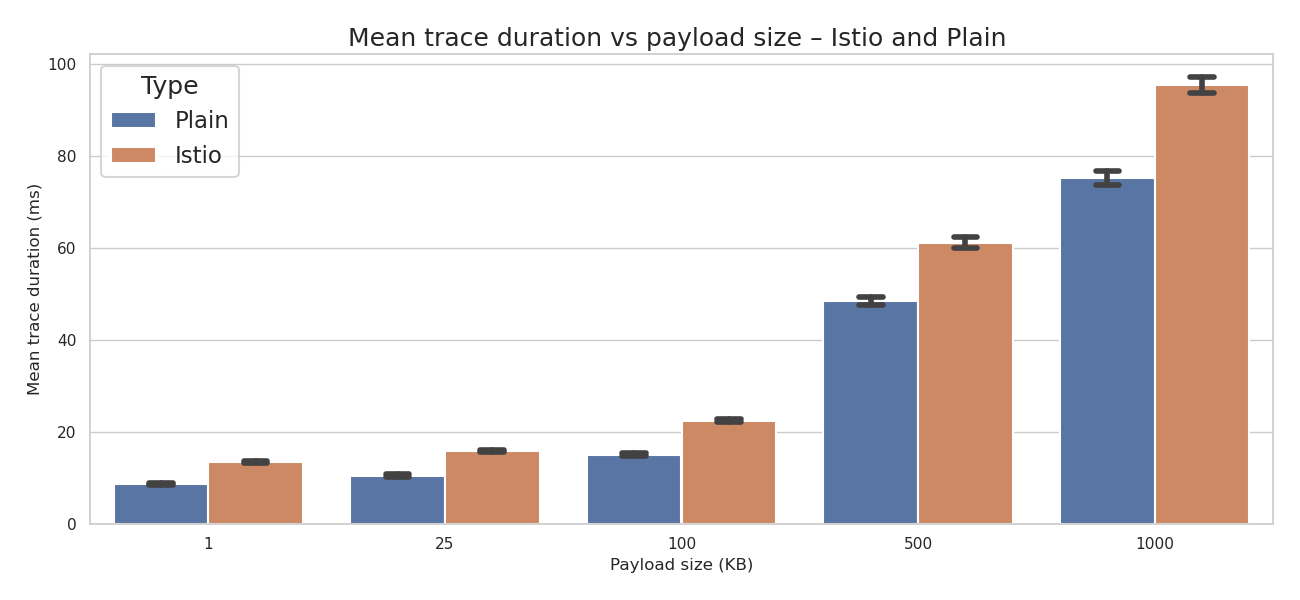
\includegraphics[
      width=\linewidth,            % never wider than text block
      height=0.8\textheight,       % never taller than 80 % of the text body
      keepaspectratio              % obey aspect ratio
  ]{img/mean_trace_duration_vs_payload.png}
  \caption{Столбчатая диаграмма среднего времени спана в зависимости от размера запроса. }
  \label{pic:mean_trace_duration_vs_payload}
\end{figure}

 \begin{figure}[htbp]
  \centering
  
  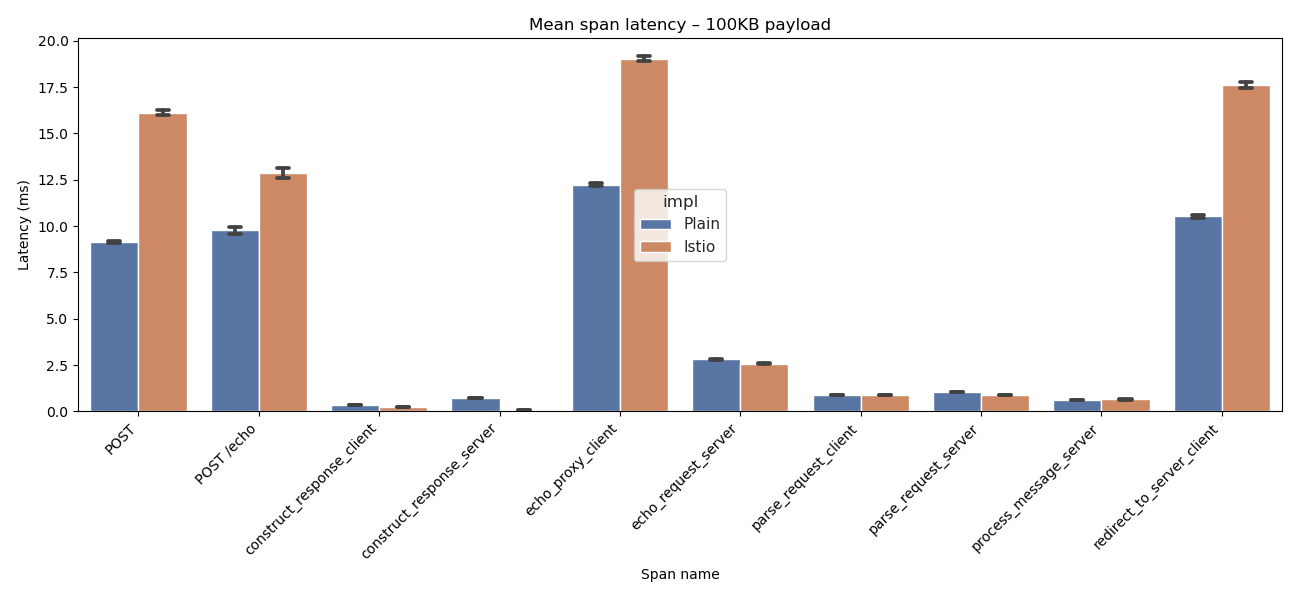
\includegraphics[
      width=\linewidth,            % never wider than text block
      height=0.8\textheight,       % never taller than 80 % of the text body
      keepaspectratio              % obey aspect ratio
  ]{img/span_latency_100kb.png}
  \caption{Диаграмма среднего времени выполнения отдельных спанов для запросов с полезной нагрузкой 100 КБ.}
  \label{pic:span_latency_100kb}
\end{figure}

\section{Выводы}
Проведённые испытания подтвердили преимущество кастомной реализации паттерна Circuit Breaker над реализацией на базе Istio с точки зрения сетевых задержек. Снижение задержек примерно на 20\% делает пользовательское решение предпочтительным для приложений, чувствительных к производительности и сетевым взаимодействиям. При этом затраты времени на выполнение внутренних вычислений остаются одинаковыми, что свидетельствует о стабильности и предсказуемости обеих реализаций. Полученные данные позволяют рекомендовать разработанную библиотеку для использования в ситуациях, где важна минимизация задержек и требуется упрощённая инфраструктура без дополнительных накладных расходов, характерных для Service Mesh решений.

Предполагается дальнейшее развитие библиотеки за счёт интеграции других паттернов отказоустойчивости, а также её последующая интеграция в проект KubeSmart — интеллектуальную систему оркестрации Docker-контейнеров для платформы PaaS, разрабатываемую лабораторией искусственного интеллекта и больших данных НИЯУ МИФИ под руководством Ровнягина М. М.
%%% Local Variables:
%%% TeX-engine: xetex
%%% eval: (setq-local TeX-master (concat "../" (seq-find (-cut string-match ".*-3-pz\.tex$" <>) (directory-files ".."))))
%%% End:
